% Fig 5:fig7 -- Distribucion del corpus por las 4 fuentes (pie chart TikZ).
% Datos reales del corpus completo (40,974 docs, ene-6abr 2026):
%   Noticias digitales 36.1% (RPP 14.1 + Correo 13.6 + Comercio 5.9 + Republica 2.5)
%   X/Twitter 37.8% | TikTok 16.3% | YouTube 9.8%
% Angulos (1% = 3.6 grados), inicio 90, sentido horario:
%   Noticias 36.1% -> 130.0  : 90 a -40.0
%   Twitter  37.8% -> 136.1  : -40.0 a -176.1
%   TikTok   16.3% ->  58.7  : -176.1 a -234.7
%   YouTube   9.8% ->  35.3  : -234.7 a -270 (=90)
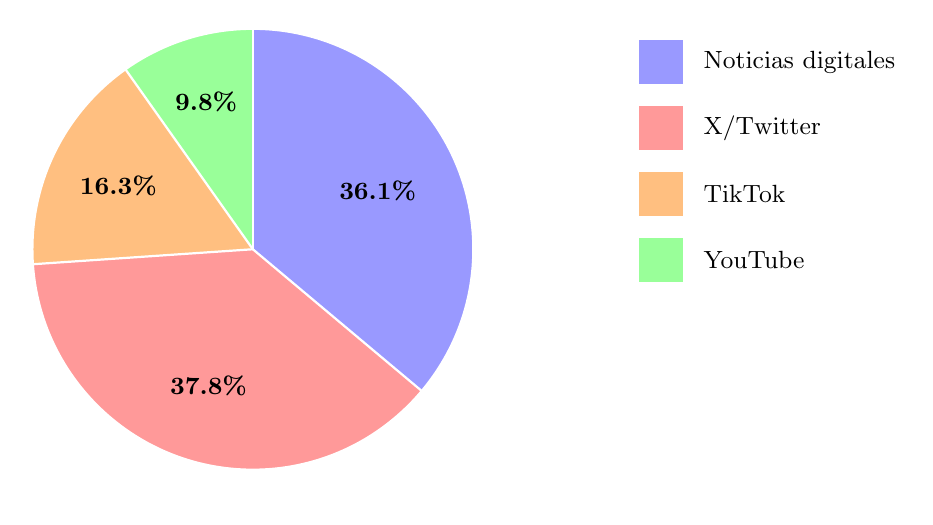
\begin{tikzpicture}[scale=1.4]
    \fill[blue!40]   (0,0) -- (90:2)     arc (90:-40:2)       -- cycle;
    \fill[red!40]    (0,0) -- (-40:2)    arc (-40:-176.1:2)   -- cycle;
    \fill[orange!50] (0,0) -- (-176.1:2) arc (-176.1:-234.7:2) -- cycle;
    \fill[green!40]  (0,0) -- (-234.7:2) arc (-234.7:-270:2)  -- cycle;

    \draw[thick, white] (0,0) circle (2);
    \foreach \a in {90,-40,-176.1,-234.7} {
        \draw[thick, white] (0,0) -- (\a:2);
    }

    % Etiquetas en el punto medio de cada sector
    \node[font=\small\bfseries] at (25:1.25)     {36.1\%};
    \node[font=\small\bfseries] at (-108:1.3)    {37.8\%};
    \node[font=\small\bfseries] at (-205.4:1.35) {16.3\%};
    \node[font=\small\bfseries] at (-252.4:1.4)  {9.8\%};

    % Leyenda
    \begin{scope}[shift={(3.5,1.5)}]
        \fill[blue!40]   (0,0)    rectangle (0.4,0.4);
        \fill[red!40]    (0,-0.6) rectangle (0.4,-0.2);
        \fill[orange!50] (0,-1.2) rectangle (0.4,-0.8);
        \fill[green!40]  (0,-1.8) rectangle (0.4,-1.4);
        \node[anchor=west, font=\small] at (0.5, 0.2)  {Noticias digitales};
        \node[anchor=west, font=\small] at (0.5,-0.4) {X/Twitter};
        \node[anchor=west, font=\small] at (0.5,-1.0) {TikTok};
        \node[anchor=west, font=\small] at (0.5,-1.6) {YouTube};
    \end{scope}
\end{tikzpicture}
